\documentclass[10pt]{article}
\usepackage[utf8]{inputenc}
\usepackage[T1]{fontenc}
\usepackage{amsmath}
\usepackage{amsfonts}
\usepackage{amssymb}
\usepackage[version=4]{mhchem}
\usepackage{stmaryrd}
\usepackage{bbold}
\usepackage{graphicx}
\usepackage[export]{adjustbox}
\graphicspath{ {./images/} }

\begin{document}
\section*{MATHEMATICS}
\section*{SECTION-A}
\begin{enumerate}
  \setcounter{enumi}{60}
  \item The statement \(\mathrm{B} \Rightarrow((\sim \mathrm{A}) \vee \mathrm{B})\) is equivalent to :\\
(1) \(\mathrm{B} \Rightarrow(\mathrm{A} \Rightarrow \mathrm{B})\)\\
(2) \(A \Rightarrow(A \Leftrightarrow B)\)\\
(3) \(\mathrm{A} \Rightarrow((\sim \mathrm{A}) \Rightarrow \mathrm{B})\)\\
(4) \(\mathrm{B} \Rightarrow((\sim \mathrm{A}) \Rightarrow \mathrm{B})\)
\end{enumerate}

Official Ans. by NTA (2)\\
Allen Ans. (1 or 3 or 4)\\
Sol.

\begin{center}
\begin{tabular}{|c|c|c|c|c|}
\hline
A & B & \(\sim \mathrm{A}\) & \(\sim \mathrm{A} \vee \mathrm{B}\) & \(\mathrm{B} \Rightarrow((\sim \mathrm{A}) \vee \mathrm{B})\) \\
\hline
T & T & F & T & T \\
\hline
T & F & F & F & T \\
\hline
F & T & T & T & T \\
\hline
F & F & T & T & T \\
\hline
\end{tabular}
\end{center}

\begin{center}
\begin{tabular}{|c|c|c|c|c|}
\hline
\(\mathrm{A} \Rightarrow \mathrm{B}\) & \(\sim \mathrm{A} \Rightarrow \mathrm{B}\) & \begin{tabular}{c}
\(\mathrm{B} \Rightarrow\) \\
\((\mathrm{A} \Rightarrow \mathrm{B})\) \\
\end{tabular} & \begin{tabular}{c}
\(\mathrm{A} \Rightarrow\) \\
\(((\sim \mathrm{A}) \Rightarrow \mathrm{B})\) \\
\end{tabular} & \begin{tabular}{c}
\(\mathrm{B} \Rightarrow\) \\
\(((\sim \mathrm{A}) \Rightarrow \mathrm{B})\) \\
\end{tabular} \\
\hline
T & T & T & T & T \\
\hline
F & T & T & T & T \\
\hline
T & T & T & T & T \\
\hline
T & F & T & T & T \\
\hline
\end{tabular}
\end{center}

\begin{enumerate}
  \setcounter{enumi}{61}
  \item Shortest distance between the lines \(\frac{x-1}{2}=\frac{y+8}{-7}=\frac{z-4}{5}\) and \(\frac{x-1}{2}=\frac{y-2}{1}=\frac{z-6}{-3}\) is\\
(1) \(2 \sqrt{3}\)\\
(2) \(4 \sqrt{3}\)\\
(3) \(3 \sqrt{3}\)\\
(4) \(5 \sqrt{3}\)
\end{enumerate}

Official Ans. by NTA (2)\\
Allen Ans. (2)

\section*{TEST PAPER WITH SOLUTION}
Sol. \(\quad \frac{x-1}{2}=\frac{y+8}{-7}=\frac{z-4}{5} \quad \vec{a}=\hat{i}-8 \hat{j}+4 \hat{k}\)\\
\(\frac{x-1}{2}=\frac{y-2}{1}=\frac{z-6}{-3} \quad \vec{b}=\hat{i}+2 \hat{j}+6 \hat{k}\)\\
\(\vec{p}=2 \hat{i}-7 \hat{j}+5 \hat{k}, \vec{q}=2 \hat{i}+\hat{j}-3 \hat{k}\)\\
\(\overrightarrow{\mathrm{p}} \times \overrightarrow{\mathrm{q}}=\left|\begin{array}{ccc}\hat{\mathrm{i}} & \hat{\mathrm{j}} & \hat{\mathrm{k}} \\ 2 & -7 & 5 \\ 2 & 1 & -3\end{array}\right|\)\\
\(=\hat{\mathrm{i}}(16)-\hat{\mathrm{j}}(-16)+\hat{\mathrm{k}}(16)\)\\
\(=16(\hat{i}+\hat{j}+\hat{k})\)\\
\(d=\left|\frac{(a-b) \cdot(\vec{p} \times \vec{q})}{|\vec{p} \times \vec{q}|}\right|=\left|\frac{(-10 \hat{j}-2 \hat{k}) \cdot 16(\hat{i}+\hat{j}+\hat{k})}{16 \sqrt{3}}\right|\)\\
\(=\left|\frac{-12}{\sqrt{3}}\right|=4 \sqrt{3}\)\\
63. If \(\vec{a}=\hat{i}+2 \hat{k}, \vec{b}=\hat{i}+\hat{j}+\hat{k}, \vec{c}=7 \hat{i}-3 \hat{k}+4 \hat{k}\),\\
\(\overrightarrow{\mathrm{r}} \times \overrightarrow{\mathrm{b}}+\overrightarrow{\mathrm{b}} \times \overrightarrow{\mathrm{c}}=\overrightarrow{0}\) and \(\overrightarrow{\mathrm{r}} . \overrightarrow{\mathrm{a}}=0\) then \(\overrightarrow{\mathrm{r}} . \overrightarrow{\mathrm{c}}\) is equal to:\\
(1) 34\\
(2) 12\\
(3) 36\\
(4) 30

Official Ans. by NTA (1)\\
Allen Ans. (1)\\
Sol. \(\vec{r} \times \vec{b}-\vec{c} \times \vec{b}=0\)\\
\(\Rightarrow(\overrightarrow{\mathrm{r}}-\overrightarrow{\mathrm{c}}) \times \overrightarrow{\mathrm{b}}=0\)\\
\(\Rightarrow \overrightarrow{\mathrm{r}}-\overrightarrow{\mathrm{c}}=\lambda \overrightarrow{\mathrm{b}}\)\\
\(\Rightarrow \overrightarrow{\mathrm{r}}=\overrightarrow{\mathrm{c}}+\lambda \overrightarrow{\mathrm{b}}\)\\
And given that \(\overrightarrow{\mathrm{r}} \cdot \overrightarrow{\mathrm{a}}=0\)\\
\(\Rightarrow(\overrightarrow{\mathrm{c}}+\lambda \overrightarrow{\mathrm{b}}) \cdot \overrightarrow{\mathrm{a}}=0\)\\
\(\Rightarrow \overrightarrow{\mathrm{c}} \cdot \overrightarrow{\mathrm{a}}+\lambda \overrightarrow{\mathrm{b}} \cdot \overrightarrow{\mathrm{a}}=0\)\\
\(\Rightarrow \lambda=\frac{-\overrightarrow{\mathrm{c}} \cdot \overrightarrow{\mathrm{a}}}{\dot{\mathrm{b}} \cdot \overrightarrow{\mathrm{a}}}\)\\
Now \(\overrightarrow{\mathrm{r}} \cdot \overrightarrow{\mathrm{c}}=(\overrightarrow{\mathrm{c}}+\lambda \overrightarrow{\mathrm{b}}) \cdot \overrightarrow{\mathrm{c}}\)

\[
\begin{aligned}
& =\left(\overrightarrow{\mathrm{c}}-\frac{\overrightarrow{\mathrm{c}} \cdot \overrightarrow{\mathrm{a}}}{\overrightarrow{\mathrm{~b}} \cdot \overrightarrow{\mathrm{a}}} \overrightarrow{\mathrm{~b}}\right) \cdot \overrightarrow{\mathrm{c}} \\
& =|\overrightarrow{\mathrm{c}}|-\left(\frac{\overrightarrow{\mathrm{c}} \cdot \overrightarrow{\mathrm{a}}}{\overrightarrow{\mathrm{~b}} \cdot \overrightarrow{\mathrm{a}}}\right)(\overrightarrow{\mathrm{b}} \cdot \overrightarrow{\mathrm{c}}) \\
& =74-\left[\frac{15}{3}\right] 8 \\
& =74-40=34
\end{aligned}
\]

\begin{enumerate}
  \setcounter{enumi}{63}
  \item Let \(S=\left\{w_{1}, w_{2}, \ldots.\right\}\) be the sample space associated to a random experiment. Let \(\mathrm{P}\left(\mathrm{w}_{\mathrm{n}}\right)=\frac{\mathrm{P}\left(\mathrm{w}_{\mathrm{n}-1}\right)}{2}, n \geq 2\). Let \(\mathrm{A}=\{2 \mathrm{k}+3 \ell ; \mathrm{k}, \ell \in \mathrm{N}\}\) and \(\mathrm{B}=\left\{\mathrm{w}_{\mathrm{n}} ; \mathrm{n} \in \mathrm{A}\right\}\). Then \(\mathrm{P}(\mathrm{B})\) is equal to\\
(1) \(\frac{3}{32}\)\\
(2) \(\frac{3}{64}\)\\
(3) \(\frac{1}{16}\)\\
(4) \(\frac{1}{32}\)
\end{enumerate}

\section*{Official Ans. by NTA (2)}
\section*{Allen Ans. (2)}
Sol. Let \(\mathrm{P}\left(\mathrm{w}_{1}\right)=\lambda\) then \(\mathrm{P}\left(\mathrm{w}_{2}\right)=\frac{\lambda}{2} \ldots \mathrm{P}\left(\mathrm{w}_{\mathrm{n}}\right)=\frac{\lambda}{2^{\mathrm{n}-1}}\)\\
As \(\sum_{\mathrm{k}=1}^{\infty} \mathrm{P}\left(\mathrm{w}_{\mathrm{k}}\right)=1 \Rightarrow \frac{\lambda}{1-\frac{1}{2}}=1 \Rightarrow \lambda=\frac{1}{2}\)\\
So, \(\mathrm{P}\left(\mathrm{w}_{\mathrm{n}}\right)=\frac{1}{2^{\mathrm{n}}}\)\\
\(\mathrm{A}=\{2 \mathrm{k}+3 \ell ; \mathrm{k}, \ell \in \mathbb{N}\}=\{5,7,8,9,10 \ldots \ldots\}\)\\
\(B=\left\{w_{n}: n \in A\right\}\)\\
\(B=\left\{W_{5}, W_{7}, W_{8}, W_{9}, W_{10}, W_{11}, \ldots\right\}\)\\
\(\mathrm{A}=\mathrm{N}-\{1,2,3,4,6\}\)\\
\(\therefore \mathrm{P}(\mathrm{B})=1-\left[\mathrm{P}\left(\mathrm{w}_{1}\right)+\mathrm{P}\left(\mathrm{w}_{2}\right)+\mathrm{P}\left(\mathrm{w}_{3}\right)+\mathrm{P}\left(\mathrm{w}_{4}\right)+\mathrm{P}\left(\mathrm{w}_{6}\right)\right]\)\\
\(=1-\left[\frac{1}{2}+\frac{1}{4}+\frac{1}{8}+\frac{1}{16}+\frac{1}{64}\right]\)\\
\(=1-\frac{32+16+8+4+1}{64}=\frac{3}{64}\)\\
65. The value of the integral \(\int_{1}^{2}\left(\frac{t^{4}+1}{t^{6}+1}\right) d t\) is :\\
(1) \(\tan ^{-1} \frac{1}{2}+\frac{1}{3} \tan ^{-1} 8-\frac{\pi}{3}\)\\
(2) \(\tan ^{-1} 2-\frac{1}{3} \tan ^{-1} 8+\frac{\pi}{3}\)\\
(3) \(\tan ^{-1} 2+\frac{1}{3} \tan ^{-1} 8-\frac{\pi}{3}\)\\
(4) \(\tan ^{-1} \frac{1}{2}-\frac{1}{3} \tan ^{-1} 8+\frac{\pi}{3}\)

Official Ans. by NTA (3)\\
Allen Ans. (3)

Sol. \(I=\int_{1}^{2}\left(\frac{t^{4}+1}{t^{6}+1}\right) d t\)\\
\(=\int_{1}^{2} \frac{\left(t^{4}+1-t^{2}\right)+t^{2}}{\left(t^{2}+1\right)\left(t^{4}-t^{2}+1\right)} d t\)\\
\(=\int_{1}^{2}\left(\frac{1}{\mathrm{t}^{2}+1}+\frac{\mathrm{t}^{2}}{\mathrm{t}^{6}+1}\right) \mathrm{dt}\)\\
\(=\int_{1}^{2}\left(\frac{1}{t^{2}+1}+\frac{1}{3} \frac{3 t^{2}}{\left(t^{3}\right)^{2}+1}\right) d t\)\\
\(=\tan ^{-1}(\mathrm{t})+\left.\frac{1}{3} \tan ^{-1}\left(\mathrm{t}^{3}\right)\right|_{1} ^{2}\)\\
\(=\left(\tan ^{-1}(2)-\tan ^{-1}(1)\right)+\frac{1}{3}\left(\tan ^{-1}\left(2^{3}\right)-\tan ^{-1}\left(1^{3}\right)\right)\)\\
\(=\tan ^{-1}(2)+\frac{1}{3} \tan ^{-1}(8)-\frac{\pi}{3}\)\\
66. Let K be the sum of the coefficients of the odd powers of x in the expansion of \((1+\mathrm{x})^{99}\). Let a be the middle term in the expansion of \(\left(2+\frac{1}{\sqrt{2}}\right)^{200}\). If \(\frac{{ }^{200} \mathrm{C}_{99} \mathrm{~K}}{\mathrm{a}}=\frac{2^{\ell} \mathrm{m}}{\mathrm{n}}\), where m and n are odd numbers, then the ordered pair \((\square, \mathrm{n})\) is equal to :\\
(1) \((50,51)\)\\
(2) \((51,99)\)\\
(3) \((50,101)\)\\
(4) \((51,101)\)

Official Ans. by NTA (3)

Allen Ans. (3)

Sol. In the expansion of\\
\((1+\mathrm{x})^{99}=\mathrm{C}_{0}+\mathrm{C}_{1} \mathrm{x}+\mathrm{C}_{2} \mathrm{x}^{2}+\ldots .+\mathrm{C}_{99} \mathrm{x}^{99}\)\\
\(\mathrm{K}=\mathrm{C}_{1}+\mathrm{C}_{3}+\ldots .+\mathrm{C}_{99}=2^{98}\)\\
\(\mathrm{a} \Rightarrow\) Middle in the expansion of \(\left(2+\frac{1}{\sqrt{2}}\right)^{200}\)\\
\(\mathrm{T}_{\frac{200}{2}+1}={ }^{200} \mathrm{C}_{100}(2)^{100}\left(\frac{1}{\sqrt{2}}\right)^{100}\)

\[
={ }^{200} \mathrm{C}_{100} .2^{50}
\]

So, \(\frac{{ }^{200} \mathrm{C}_{99} \times 2^{98}}{{ }^{200} \mathrm{C}_{100} \times 2^{50}}=\frac{100}{101} \times 2^{48}\)\\
So, \(\frac{25}{101} \times 2^{50}=\frac{\mathrm{m}}{\mathrm{n}} 2^{\ell}\)\\
\(\therefore \mathrm{m}, \mathrm{n}\) are odd so\\
( \(\square, \mathrm{n}\) ) become \((50,101)\) Ans.\\
67. Let \(f\) and \(g\) be twice differentiable functions on \(R\) such that\\
\(\mathrm{f}^{\prime \prime}(\mathrm{x})=\mathrm{g}^{\prime \prime}(\mathrm{x})+6 \mathrm{x}\)\\
\(\mathrm{f}^{\prime}(1)=4 \mathrm{~g}^{\prime}(1)-3=9\)\\
\(\mathrm{f}(2)=3 \mathrm{~g}(2)=12\)\\
Then which of the following is NOT true ?\\
(1) \(\mathrm{g}(-2)-\mathrm{f}(-2)=20\)\\
(2) If \(-1<\mathrm{x}<2\), then \(|\mathrm{f}(\mathrm{x})-\mathrm{g}(\mathrm{x})|<8\)\\
(3) \(\left|\mathrm{f}^{\prime}(\mathrm{x})-\mathrm{g}^{\prime}(\mathrm{x})\right|<6 \Rightarrow-1<\mathrm{x}<1 \mid\)\\
(4) There exists \(x_{0} \in\left(1, \frac{3}{2}\right)\) such that \(f\left(x_{0}\right)=g\left(x_{0}\right)\)

Official Ans. by NTA (2)\\
Allen Ans. (2)\\
Sol. \(\mathrm{f}^{\prime \prime}(\mathrm{x})=\mathrm{g}^{\prime \prime}(\mathrm{x})+6 \mathrm{x}\)\\
\(\mathrm{f}^{\prime}(1)=4 \mathrm{~g}^{\prime}(1)-3=9\)\\
\(\mathrm{f}(2)=3 \mathrm{~g}(2)=12\)

By integrating (1)

\[
f^{\prime}(x)=g^{\prime}(x)+6 \frac{x^{2}}{2}+C
\]

At \(\mathrm{x}=1\),

\[
\begin{gathered}
f^{\prime}(1)=g^{\prime}(1)+3+C \\
\Rightarrow 9=4+3+C \Rightarrow C=3
\end{gathered}
\]

\(\therefore \quad \mathrm{f}^{\prime}(\mathrm{x})=\mathrm{g}^{\prime}(\mathrm{x})+3 \mathrm{x}^{2}+3\)\\
Again by integrating,\\
\(f(x)=g(x)+\frac{3 x^{3}}{3}+3 x+D\)\\
At \(\mathrm{x}=2\),\\
\(\mathrm{f}(2)=\mathrm{g}(2)+8+3(2)+\mathrm{D}\)\\
\(\Rightarrow 12=4+8+6+D \Rightarrow D=-6\)\\
So, \(f(x)=g(x)+x^{3}+3 x-6\)\\
\(\Rightarrow \mathrm{f}(\mathrm{x})-\mathrm{g}(\mathrm{x})=\mathrm{x}^{3}+3 \mathrm{x}-6\)\\
At \(\mathrm{x}=-2\),\\
\(\Rightarrow \mathrm{g}(-2)-\mathrm{f}(-2)=20 \quad\) (Option (1) is true)\\
Now, for \(-1<\mathrm{x}, 2\)\\
\(h(x)=f(x)-g(x)=x^{3}+3 x-6\)\\
\(\Rightarrow \mathrm{h}^{\prime}(\mathrm{x})=3 \mathrm{x}^{2}+3\)\\
\(\Rightarrow \mathrm{h}(\mathrm{x}) \uparrow\)\\
So, \(\mathrm{h}(-1)<\mathrm{h}(\mathrm{x})<\mathrm{h}(2)\)\\
\(\Rightarrow-10<\mathrm{h}(\mathrm{x})<8\)\\
\(\Rightarrow|\mathrm{h}(\mathrm{x})|<10 \quad\) (option (2) is NOT true)\\
Now, \(\mathrm{h}^{\prime}(\mathrm{x})=\mathrm{f}^{\prime}(\mathrm{x})-\mathrm{g}^{\prime}(\mathrm{x})=3 \mathrm{x}^{2}+3\)\\
If \(\left|\mathrm{h}^{\prime}(\mathrm{x})\right|<6 \Rightarrow\left|3 \mathrm{x}^{2}+3\right|<6\)\\
\(\Rightarrow 3 \mathrm{x}^{2}+3<6\)\\
\(\Rightarrow \mathrm{x}^{2}<1\)\\
\(\Rightarrow-1<\mathrm{x}<1 \quad\) (option (3) is True)\\
If \(\mathrm{x} \in(-1,1)\left|\mathrm{f}^{\prime}(\mathrm{x})-\mathrm{g}^{\prime}(\mathrm{x})\right|<6\)\\
option (3) is true and now to solve\\
\(\mathrm{f}(\mathrm{x})-\mathrm{g}(\mathrm{x})=0\)\\
\(\Rightarrow \mathrm{x}^{3}+3 \mathrm{x}-6=0\)\\
\(h(x)=x^{3}+3 x-6\)\\
here, \(h(1)=-v e\) and \(h\left(\frac{3}{2}\right)=+v e\)\\
So there exists \(\mathrm{x}_{0} \in\left(1, \frac{3}{2}\right)\) such that \(\mathrm{f}\left(\mathrm{x}_{0}\right)=\mathrm{g}\left(\mathrm{x}_{0}\right)\)\\
(option (4) is true)\\
68. The set of all values of \(t \in \mathbb{R}\), for which the matrix

\[
\left[\begin{array}{ccc}
e^{t} & e^{-t}(\sin t-2 \cos t) & e^{-t}(-2 \sin t-\cos t) \\
e^{t} & e^{-t}(2 \sin t+\cos t) & e^{-t}(\sin t-2 \cos t) \\
e^{t} & e^{-t} \cos t & e^{-t} \sin t
\end{array}\right]
\]

is invertible, is\\
(1) \(\left\{(2 \mathrm{k}+1) \frac{\pi}{2}, \mathrm{k} \in \mathbb{Z}\right\}\)\\
(2) \(\left\{\mathrm{k} \pi+\frac{\pi}{4}, \mathrm{k} \in \mathbb{Z}\right\}\)\\
(3) \(\{\mathrm{k} \pi, \mathrm{k} \in \mathbb{Z}\}\)\\
(4) \(\mathbb{R}\)

\section*{Official Ans. by NTA (4)}
Allen Ans. (4)\\
Sol. If its invertible, then determinant value \(\neq 0\)\\
So ,\\
\(\left|\begin{array}{ccc}e^{t} & e^{-t}(\sin t-2 \cos t) & e^{-t}(-2 \sin t-\cos t) \\ e^{t} & e^{-t}(2 \sin t+\cos t) & e^{-t}(\sin t-2 \cos t) \\ e^{t} & e^{-t} \cos t & e^{-t} \sin t\end{array}\right| \neq 0\)\\
\(\Rightarrow e^{t} \cdot e^{-t} \cdot e^{-t}\left|\begin{array}{ccc}1 & \sin t-2 \cos t & -2 \sin t-\cos t \\ 1 & 2 \sin t+\cos t & \sin t-2 \cos t \\ 1 & \cos t & \sin t\end{array}\right| \neq 0\)\\
Applying, \(\mathrm{R}_{1} \rightarrow \mathrm{R}_{1}-\mathrm{R}_{2}\) then \(\mathrm{R}_{2} \rightarrow \mathrm{R}_{2}-\mathrm{R}_{3}\)\\
We get\\
\(\mathrm{e}^{-\mathrm{t}}\left|\begin{array}{ccc}0 & -\sin \mathrm{t}-\cos \mathrm{t} & -3 \sin \mathrm{t}+\cos \mathrm{t} \\ 0 & 2 \sin \mathrm{t} & -2 \cos \mathrm{t} \\ 1 & \cos \mathrm{t} & \sin \mathrm{t}\end{array}\right| \neq 0\)\\
By expanding we have,\\
\(\mathrm{e}^{-\mathrm{t}} \times 1\left(2 \sin \mathrm{t} \cos \mathrm{t}+6 \cos ^{2} \mathrm{t}+6 \sin ^{2} \mathrm{t}-2 \sin \mathrm{t} \cos \mathrm{t}\right) \neq 0\)\\
\(\Rightarrow \mathrm{e}^{-\mathrm{t}} \times 6 \neq 0\)\\
for \(\forall \mathrm{t} \in \mathbb{R}\)\\
69. The area of the region\\
\(A=\left\{(x, y):|\cos x-\sin x| \leq y \leq \sin x, 0 \leq x \leq \frac{\pi}{2}\right\}\)\\
(1) \(1-\frac{3}{\sqrt{2}}+\frac{4}{\sqrt{5}}\)\\
(2) \(\sqrt{5}+2 \sqrt{2}-4.5\)\\
(3) \(\frac{3}{\sqrt{5}}-\frac{3}{\sqrt{2}}+1\)\\
(4) \(\sqrt{5}-2 \sqrt{2}+1\)

Official Ans. by NTA (4)\\
Allen Ans. (4)

Sol. \(|\cos x-\sin x| \leq y \leq \sin x\)\\
Intersection point of \(\cos x-\sin x=\sin x\)\\
\(\Rightarrow \tan \mathrm{x}=\frac{1}{2}\)\\
Let \(\psi=\tan ^{-1} \frac{1}{2}\)\\
So, \(\tan \psi=\frac{1}{2}, \sin \psi=\frac{1}{\sqrt{5}}, \cos \psi=\frac{2}{\sqrt{5}}\)\\
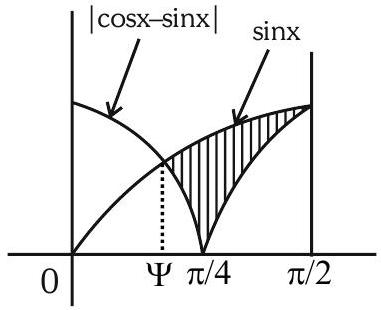
\includegraphics[max width=\textwidth, center]{2025_10_03_52c1403254efafd0f70bg-04}

\[
\begin{aligned}
\text { Area }= & \int_{\psi}^{\pi / 2}(\sin x-|\cos x-\sin x|) d x \\
= & \int_{\psi}^{\pi / 4}(\sin x-(\cos x-\sin x)) d x \\
& \quad+\int_{\pi / 4}^{\pi / 2}(\sin x-(\sin x-\cos x)) d x \\
= & \int_{\psi}^{\pi / 4}(2 \sin x-\cos x) d x+\int_{\pi / 4}^{\pi / 2} \cos x d x \\
= & {[-2 \cos x-\sin x]_{\psi}^{\pi / 4}+[\sin x]_{\pi / 4}^{\pi / 2} } \\
= & -\sqrt{2}-\frac{1}{\sqrt{2}}+2 \cos \psi+\sin \psi+\left(1-\frac{1}{\sqrt{2}}\right) \\
= & -\sqrt{2}-\frac{1}{\sqrt{2}}+2\left(\frac{2}{\sqrt{5}}\right)+\left(\frac{1}{\sqrt{5}}\right)+1-\frac{1}{\sqrt{2}} \\
= & \sqrt{5}-2 \sqrt{2}+1
\end{aligned}
\]

\begin{enumerate}
  \setcounter{enumi}{69}
  \item The set of all values of \(\lambda\) for which the equation \(\cos ^{2} 2 x-2 \sin ^{4} x-2 \cos ^{2} x=\lambda\)\\
(1) \([-2,-1]\)\\
(2) \(\left[-2,-\frac{3}{2}\right]\)\\
(3) \(\left[-1,-\frac{1}{2}\right]\)\\
(4) \(\left[-\frac{3}{2},-1\right]\)
\end{enumerate}

Official Ans. by NTA (4)\\
Allen Ans. (4)

DIGITAL

Sol. \(\quad \lambda=\cos ^{2} 2 \mathrm{x}-2 \sin ^{4} \mathrm{x}-2 \cos ^{2} \mathrm{x}\)\\
convert all in to \(\cos \mathrm{x}\).

\[
\begin{aligned}
& \lambda=\left(2 \cos ^{2} x-1\right)^{2}-2\left(1-\cos ^{2} x\right)^{2}-2 \cos ^{2} x \\
&=4 \cos ^{4} x-4 \cos ^{2} x+1-2\left(1-2 \cos ^{2} x+\cos ^{4} x\right)- \\
& 2 \cos ^{2} x \\
&=2 \cos ^{4} x-2 \cos ^{2} x+1-2 \\
&=2 \cos ^{4} x-2 \cos ^{2} x-1 \\
&=2\left[\cos ^{4} x-\cos ^{2} x-\frac{1}{2}\right] \\
&=2\left[\left(\cos ^{2} x-\frac{1}{2}\right)^{2}-\frac{3}{4}\right] \\
& \lambda_{\max }=2\left[\frac{1}{4}-\frac{3}{4}\right]=2 \times\left(-\frac{2}{4}\right)=-1(\text { max Value }) \\
& \lambda_{\min }=2\left[0-\frac{3}{4}\right]=-\frac{3}{2}(\text { MinimumValue }) \\
& \text { So, Range }=\left[-\frac{3}{2},-1\right]
\end{aligned}
\]

\begin{enumerate}
  \setcounter{enumi}{70}
  \item The letters of the word OUGHT are written in all possible ways and these words are arranged as in a dictionary, in a series. Then the serial number of the word TOUGH is :\\
(1) 89\\
(2) 84\\
(3) 86\\
(4) 79
\end{enumerate}

Official Ans. by NTA (1)\\
Allen Ans. (1)\\
Sol. Lets arrange the letters of OUGHT in alphabetical order.

\[
\mathrm{G}, \mathrm{H}, \mathrm{O}, \mathrm{~T}, \mathrm{U}
\]

Words starting with\\
\(\mathrm{G}----\rightarrow 4\) !\\
\(\mathrm{H}----\rightarrow 4\) !\\
\(\mathrm{O}----\rightarrow 4\) !\\
T G \(---\rightarrow 3\) !\\
T H \(---\rightarrow 3\) !\\
T O G \(--\rightarrow 2\) !\\
T O H \(--\rightarrow 2\) !\\
TOUGH \(\rightarrow 1\) !

Total \(=89\)\\
72. The plane \(2 x-y+z=4\) intersects the line segment joining the points \(\mathrm{A}(\mathrm{a},-2,4)\) and \(\mathrm{B}(2, \mathrm{~b},-3)\) at the point C in the ratio \(2: 1\) and the distance of the point C from the origin is \(\sqrt{5}\). If \(\mathrm{ab}<0\) and P is the point \((\mathrm{a}-\mathrm{b}, \mathrm{b}, 2 \mathrm{~b}-\mathrm{a})\) then \(\mathrm{CP}^{2}\) is equal to:\\
(1) \(\frac{17}{3}\)\\
(2) \(\frac{16}{3}\)\\
(3) \(\frac{73}{3}\)\\
(4) \(\frac{97}{3}\)

\section*{Official Ans. by NTA (1)}
Allen Ans. (1)\\
Sol. \(\mathrm{A}(\mathrm{a},-2,4), \mathrm{B}(2, \mathrm{~b},-3)\)

\[
\begin{aligned}
& \mathrm{AC}: \mathrm{CB}=2: 1 \\
& \Rightarrow \mathrm{C} \equiv\left(\frac{\mathrm{a}+4}{3}, \frac{2 \mathrm{~b}-2}{3}, \frac{-2}{3}\right)
\end{aligned}
\]

C lies on \(2 x-y+2=4\)

\[
\begin{aligned}
& \Rightarrow \frac{2 a+8}{3}-\frac{2 b-2}{3}-\frac{2}{3}=4 \\
& \Rightarrow a-b=2 \ldots(1)
\end{aligned}
\]

Also \(\mathrm{OC}=\sqrt{5}\)

\[
\Rightarrow\left(\frac{a+4}{3}\right)^{2}+\left(\frac{2 b-2}{3}\right)^{2}+\frac{4}{9}=5
\]

Solving, (1) and (2)

\[
\begin{aligned}
& (b+6)^{2}+(2 b-2)^{2}=41 \\
\Rightarrow & 5 b^{2}+4 b-1=0 \\
\Rightarrow & b=-1 \text { or } \frac{1}{5} \\
\Rightarrow & a=1 \text { or } \frac{11}{5}
\end{aligned}
\]

But \(\mathrm{ab}<0 \Rightarrow(\mathrm{a}, \mathrm{b})=(1,-1)\)\\
\(\mathrm{C} \equiv\left(\frac{5}{3}, \frac{-4}{3}, \frac{-2}{3}\right), \mathrm{P} \equiv(2,-1,-3)\)\\
\(\mathrm{CP}^{2}=\frac{1}{9}+\frac{1}{9}+\frac{49}{9}=\frac{51}{9}=\frac{17}{3}\)\\
73. Let \(\vec{a}=4 \hat{i}+3 \hat{j}\) and \(\vec{b}=3 \hat{i}-4 \hat{j}+5 \hat{k}\) and \(\vec{c}\) is a vector such that \(\vec{c} \cdot(\vec{a} \times \vec{b})+25=0, \vec{c} \cdot(\hat{i}+\hat{j}+\hat{k})=4\) and projection of \(\overrightarrow{\mathrm{c}}\) on \(\overrightarrow{\mathrm{a}}\) is 1 , then the projection of \(\vec{c}\) on \(\vec{b}\) equals:\\
(1) \(\frac{5}{\sqrt{2}}\)\\
(2) \(\frac{1}{5}\)\\
(3) \(\frac{1}{\sqrt{2}}\)\\
(4) \(\frac{3}{\sqrt{2}}\)

Official Ans. by NTA (1)\\
Allen Ans. (1)\\
Sol. \(\quad \vec{a} \times \vec{b}=15 \hat{i}-20 \hat{j}-25 \hat{k}\)\\
Let \(\vec{c}=x \hat{i}+y \hat{j}+z \hat{k}\)

\[
\begin{aligned}
& \Rightarrow \quad 15 x-20 y-25 z+25=0 \\
& \Rightarrow \quad 3 x-4 y-5 z=-5
\end{aligned}
\]

Also \(\mathrm{x}+\mathrm{y}+\mathrm{z}=4\)\\
and \(\frac{\overrightarrow{\mathrm{c}} \cdot \overrightarrow{\mathrm{a}}}{|\overrightarrow{\mathrm{a}}|}=1 \Rightarrow 4 \mathrm{x}+3 \mathrm{y}=5\)

\[
\Rightarrow \quad \vec{c}=2 \hat{i}-\hat{j}+3 \hat{k}
\]

Projection of \(\vec{c}\) or \(\vec{b}=\frac{25}{5 \sqrt{2}}=\frac{5}{\sqrt{2}}\)\\
74. If the lines \(\frac{x-1}{1}=\frac{y-2}{2}=\frac{z+3}{1}\) and \(\frac{x-a}{2}=\frac{y+2}{3}=\frac{z-3}{1}\) intersects at the point \(P\), then the distance of the point P from the plane \(\mathrm{z}=\mathrm{a}\) is :\\
(1) 16\\
(2) 28\\
(3) 10\\
(4) 22

Official Ans. by NTA (2)\\
Allen Ans. (2)

Sol. Point on \(\mathrm{L}_{1} \equiv(\lambda+1,2 \lambda+2, \lambda-3)\)\\
Point on \(\mathrm{L}_{2} \equiv(2 \mu+\mathrm{a}, 3 \mu-2, \mu+3)\)

\[
\begin{array}{ll}
\lambda-3=\mu+3 & \Rightarrow \lambda=\mu+6 \\
2 \lambda+2=3 \mu-2 & \Rightarrow 2 \lambda=3 \mu-4
\end{array}
\]

Solving, (1) and (2)

\[
\begin{array}{ll}
\Rightarrow & \lambda=22 \& \mu=16 \\
\Rightarrow & \mathrm{P} \equiv(23,46,19) \\
\Rightarrow & \mathrm{a}=-9
\end{array}
\]

Distance of P from \(\mathrm{z}=-9\) is 28\\
75. The value of the integral \(\int_{1 / 2}^{2} \frac{\tan ^{-1} x}{x} d x\) is equal to\\
(1) \(\pi \log _{e} 2\)\\
(2) \(\frac{1}{2} \log _{\mathrm{e}} 2\)\\
(3) \(\frac{\pi}{4} \log _{e} 2\)\\
(4) \(\frac{\pi}{2} \log _{e} 2\)

Official Ans. by NTA (4)\\
Allen Ans. ( 4)\\
Sol. \(\quad \mathrm{I}=\int_{1 / 2}^{2} \frac{\tan ^{-1} \mathrm{x}}{\mathrm{x}} \mathrm{dx}\)

Put \(\quad \mathrm{x}=\frac{1}{\mathrm{t}} \quad \mathrm{dx}=-\frac{1}{\mathrm{t}^{2}} \mathrm{dt}\)

\[
\begin{aligned}
& I=-\int_{2}^{1 / 2} \frac{\tan ^{-1} \frac{1}{t}}{\frac{1}{t}} \cdot \frac{1}{t^{2}} d t=-\int_{2}^{1 / 2} \frac{\tan ^{-1} \frac{1}{t}}{t} d t \\
& I=\int_{1 / 2}^{2} \frac{\cot ^{-1} t}{t} d t=\int_{1 / 2}^{2} \frac{\cot ^{-1} x}{x} d x \ldots \ldots
\end{aligned}
\]

Add both equation

\[
\begin{aligned}
2 \mathrm{I}= & \int_{1 / 2}^{2} \frac{\tan ^{-1} \mathrm{x}+\cot ^{-1} \mathrm{x}}{\mathrm{x}} \mathrm{dx}=\frac{\pi}{2} \int_{1 / 2}^{2} \frac{\mathrm{dx}}{\mathrm{x}}=\frac{\pi}{2}(\ln 2)_{1 / 2}^{2} \\
& =\frac{\pi}{2}\left(\ln 2-\ell \mathrm{n} \frac{1}{2}\right)=\pi \ell \mathrm{n} 2 \\
& \mathrm{I}=\frac{\pi}{2} \ell \mathrm{n} 2
\end{aligned}
\]

\begin{enumerate}
  \setcounter{enumi}{75}
  \item If the tangent at a point P on the parabola \(\mathrm{y}^{2}=3 \mathrm{x}\) is parallel to the line \(x+2 y=1\) and the tangents at the points \(Q\) and \(R\) on the ellipse \(\frac{x^{2}}{4}+\frac{y^{2}}{1}=1\) are perpendicular to the line \(\mathrm{x}-\mathrm{y}=2\), then the area of the triangle PQR is:\\
(1) \(\frac{9}{\sqrt{5}}\)\\
(2) \(5 \sqrt{3}\)\\
(3) \(\frac{3}{2} \sqrt{5}\)\\
(4) \(3 \sqrt{5}\)
\end{enumerate}

Official Ans. by NTA (4)\\
Allen Ans. (4)

Sol. \(y^{2}=3 x\)\\
Tangent \(\mathrm{P}\left(\mathrm{x}_{1}, \mathrm{y}_{1}\right)\) is parallel to \(\mathrm{x}+2 \mathrm{y}=1\)\\
Then slope at \(\mathrm{P}=-\frac{1}{2}\)\\
\(2 y \frac{d y}{d x}=3\)\\
\(\Rightarrow \frac{\mathrm{dy}}{\mathrm{dx}}=\frac{3}{2 \mathrm{y}}=-\frac{1}{2}\)\\
\(\Rightarrow y_{1}=-3\)\\
Coordinates of \(\mathrm{P}(3,-3)\)\\
Similarly \(\mathrm{Q}\left(\frac{4}{\sqrt{3}}, \frac{1}{\sqrt{5}}\right), \mathrm{R}\left(-\frac{4}{\sqrt{5}}, \frac{-1}{\sqrt{5}}\right)\)\\
Area of \(\triangle \mathrm{PQR}\)

\[
\begin{aligned}
& =\frac{1}{2}\left|\begin{array}{ccc}
3 & -3 & 1 \\
\frac{4}{\sqrt{5}} & \frac{1}{\sqrt{5}} & 1 \\
-\frac{4}{\sqrt{5}} & -\frac{1}{\sqrt{5}} & 1
\end{array}\right| \\
& =\frac{1}{2}\left[3\left(\frac{2}{\sqrt{5}}\right)+3\left(\frac{8}{\sqrt{5}}\right)+0\right]=\frac{30}{2 \sqrt{5}}=3 \sqrt{5}
\end{aligned}
\]

\begin{enumerate}
  \setcounter{enumi}{76}
  \item Let \(y=y(x)\) be the solution of the differential equation \(\quad x \log _{e} x \frac{d y}{d x}+y=x^{2} \log _{e} x,(x>1) . \quad\) If \(y(2)=2\), then \(y(e)\) is equal to\\
(1) \(\frac{4+e^{2}}{4}\)\\
(2) \(\frac{1+\mathrm{e}^{2}}{4}\)\\
(3) \(\frac{2+\mathrm{e}^{2}}{2}\)\\
(4) \(\frac{1+\mathrm{e}^{2}}{2}\)
\end{enumerate}

Official Ans. by NTA (1)\\
Allen Ans. (1)

Sol. \(\quad x \log _{e} x \frac{d y}{d x}+y=x^{2} \log _{e} x,(x>1)\).\\
\(\Rightarrow \frac{d y}{d x}+\frac{y}{x \ln x}=x\)\\
Linear differential equation

\[
\text { I.F. }=e^{\int \frac{1}{x \ln x} d x}=|\ln x|
\]

\(\therefore\) Solution of differential equation

\[
\begin{aligned}
y|\ln x| & =\int x|\ln x| d x \\
& =|\ln x| \frac{x^{2}}{2}-\int \frac{1}{x} \cdot \frac{x^{2}}{2} d x \\
\Rightarrow y|\ln x| & =|\ln x|\left(\frac{x^{2}}{2}\right)-\frac{x^{2}}{4}+c
\end{aligned}
\]

For constant

\[
y(2)=2 \Rightarrow c=1
\]

So, \(y(x)=\frac{x^{2}}{2}-\frac{x^{2}}{4|\ln x|}+\frac{1}{|\ln x|}\)\\
Hence, \(y(e)=\frac{e^{2}}{2}-\frac{e^{2}}{4}+1=1+\frac{e^{2}}{4}\)\\
78. The number of 3 digit numbers, that are divisible by either 3 or 4 but not divisible by 48 , is\\
(1) 472\\
(2) 432\\
(3) 507\\
(4) 400

Official Ans. by NTA (2)\\
Allen Ans. (2)\\
Sol. \(\quad\) Total 3 digit number \(=900\)\\
\(\begin{array}{ll}\text { Divisible by } 3=300 & \left(\text { Using } \frac{900}{3}=300\right) \\ \text { Divisible by } 4=225 & \left(\text { Using } \frac{900}{4}=225\right)\end{array}\)\\
Divisible by \(3 \& 4=108, \ldots\).

\[
\left(\text { Using } \frac{900}{12}=75\right)
\]

Number divisible by either 3 or 4

\[
=300+2250-75=450
\]

We have to remove divisible by 48,

\[
144,192, \ldots \ldots, 18 \text { terms }
\]

Required number of numbers \(=450-18=432\)\\
79. Let \(R\) be a relation defined on \(N\) as a \(R b\) is \(2 \mathrm{a}+3 \mathrm{~b}\) is a multiple of \(5, \mathrm{a}, \mathrm{b} \in \mathbb{N}\). Then R is\\
(1) not reflexive\\
(2) transitive but not symmetric\\
(3) symmetric but not transitive\\
(4) an equivalence relation

Official Ans. by NTA (4)\\
Allen Ans. (4)\\
Sol. a \(\mathrm{R} \mathrm{a} \Rightarrow 5 \mathrm{a}\) is multiple it 5\\
So reflexive\\
\(\mathrm{a} R \mathrm{~b} \Rightarrow 2 \mathrm{a}+3 \mathrm{~b}=5 \alpha\),\\
Now b R a

\[
\begin{aligned}
2 b+3 a & =2 b+\left(\frac{5 \alpha-3 b}{2}\right) \cdot 3 \\
& =\frac{15}{2} \alpha-\frac{5}{2} b=\frac{5}{2}(3 \alpha-b) \\
& =\frac{5}{2}(2 a+2 b-2 \alpha) \\
& =5(a+b-\alpha)
\end{aligned}
\]

Hence symmetric\\
\(\mathrm{aRb} \quad \Rightarrow \quad 2 \mathrm{a}+3 \mathrm{~b}=5 \alpha\).\\
\(\mathrm{bRc} \quad \Rightarrow \quad 2 \mathrm{~b}+3 \mathrm{c}=5 \beta\)\\
Now \(\quad 2 \mathrm{a}+5 \mathrm{~b}+3 \mathrm{c}=5(\alpha+\beta)\)\\
\(\Rightarrow 2 \mathrm{a}+5 \mathrm{~b}+3 \mathrm{c}=5(\alpha+\beta)\)\\
\(\Rightarrow 2 \mathrm{a}+3 \mathrm{c}=5(\alpha+\beta-\mathrm{b})\)\\
\(\Rightarrow \mathrm{a} R \mathrm{c}\)\\
Hence relation is equivalence relation.\\
80. Consider a function \(\mathrm{f}: \mathbb{N} \rightarrow \mathbb{R}\), satisfying\\
\(f(1)+2 f(2)+3 f(3)+\ldots+x f(x)=x(x+1) f(x) ; x \geq 2\) with \(f(1)=1\). Then \(\frac{1}{f(2022)}+\frac{1}{f(2028)}\) is equal to\\
(1) 8200\\
(2) 8000\\
(3) 8400\\
(4) 8100

Official Ans. by NTA (4)\\
Allen Ans. (4)

Sol. Given for \(\mathrm{x} \geq 2\)

\[
f(1)+2 f(2)+\ldots . .+x f(x)=x(x+1) f(x)
\]

replace x by \(\mathrm{x}+1\)

\[
\begin{aligned}
& \Rightarrow \quad x(x+1) f(x)+(x+1) f(x+1) \\
& \Rightarrow \quad \frac{x}{f(x+1)}+\frac{1}{f(x)}=\frac{(x+2)}{f(x)} \\
& \Rightarrow \quad x f(x)=(x+1) f(x+1)=\frac{1}{2}, x \geq 2 \\
& f(2)=\frac{1}{4}, f(3)=\frac{1}{6}
\end{aligned}
\]

Now \(f(2022)=\frac{1}{4044}\)

\[
f(2028)=\frac{1}{4056}
\]

So, \(\frac{1}{f(2022)}+\frac{1}{f(2028)}=4044+4056=8100\)

\section*{SECTION-B}
\begin{enumerate}
  \setcounter{enumi}{80}
  \item The total number of 4-digit numbers whose greatest common divisor with 54 is 2 , is \(\_\_\_\_\) .
\end{enumerate}

Official Ans. by NTA (3000)

\section*{Allen Ans. (3000)}
Sol. N should be divisible by 2 but not by 3\\
\(\mathrm{N}=(\) Numbers divisible by 2\()-(\) Numbers divisible by 6 )\\
\(\mathrm{N}=\frac{9000}{2}-\frac{9000}{6}=4500-1500=3000\)\\
82. A triangle is formed by the tangents at the point \((2,2)\) on the curves \(y^{2}=2 x\) and \(x^{2}+y^{2}=4 x\), and the line \(\mathrm{x}+\mathrm{y}+2=0\). If r is the radius of its circumcircle, then \(\mathrm{r}^{2}\) is equal to \(\_\_\_\_\) .

Official Ans. by NTA (10)\\
Allen Ans. (10)

Sol. \(\mathrm{S}_{1}: \mathrm{y}^{2}=2 \mathrm{x} \quad \mathrm{S}_{2}: \mathrm{x}^{2}+\mathrm{y}^{2}=4 \mathrm{x}\)\\
\(\mathrm{P}(2,2)\) is common point on \(\mathrm{S}_{1} \& \mathrm{~S}_{2}\)\\
\(\mathrm{T}_{1}\) is tangent to \(\mathrm{S}_{1}\) at \(\mathrm{P} \quad \Rightarrow \mathrm{T}_{1}: \mathrm{y} \cdot 2=\mathrm{x}+2\)

\[
\Rightarrow \mathrm{T}_{1}: \mathrm{x}-2 \mathrm{y}+2=0
\]

\(\mathrm{T}_{2}\) is tangent to \(\mathrm{S}_{2}\) at \(\mathrm{P} \quad \Rightarrow \mathrm{T}_{2}: \mathrm{x} .2+\mathrm{y} .2=2(\mathrm{x}+2)\)

\[
\Rightarrow T_{2}: y=2
\]

\& \(\mathrm{L}_{3}: \mathrm{x}+\mathrm{y}+2=0\) is third line\\
\(\mathrm{PQ}=\mathrm{a}=\sqrt{20}\)\\
\(\mathrm{QR}=\mathrm{b}=\sqrt{8}\)\\
\(\mathrm{RP}=\mathrm{c}=6\)

Area \((\triangle \mathrm{PQR})=\Delta=\frac{1}{2} \times 6 \times 2=6\)\\
\(\therefore \mathrm{r}=\frac{\mathrm{abc}}{4 \Delta}=\frac{\sqrt{160}}{4}=\sqrt{10} \Rightarrow \mathrm{r}^{2}=10\)\\
83. A circle with centre \((2,3)\) and radius 4 intersects the line \(\mathrm{x}+\mathrm{y}=3\) at the points P and Q . If the tangents at P and Q intersect at the point \(\mathrm{S}(\alpha, \beta)\), then \(4 \alpha-7 \beta\) is equal to \(\_\_\_\_\) .

Official Ans. by NTA (11)

Allen Ans. (11)

Sol. The given line is polar or \(\mathrm{P}(2, \beta)\) w.r.t. given circle

\[
x^{2}+y^{2}-4 x-6 y-3=0
\]

Chord or contact\\
\(\alpha x+\beta y-2(x+\alpha)-3(y+\beta)-3=0\)

\[
\Rightarrow(\alpha-2) x+(\beta-3) y-(2 \alpha+3 \beta+3)=0
\]

\(\square\) But the equation of chord of contact is given

\[
\text { as : } x+y-3=0
\]

comparing the coefficients

\[
\frac{\alpha-2}{1}=\frac{\beta-3}{1}=-\left(\frac{2 \alpha+3 \beta+3}{-3}\right)
\]

On solving \(\alpha=-6\)

\[
\beta=-5
\]

Now

\[
4 \alpha-7 \beta=11
\]

\begin{enumerate}
  \setcounter{enumi}{83}
  \item Let \(\mathrm{a}_{1}=\mathrm{b}_{1}=1\) and \(\mathrm{a}_{\mathrm{n}}=\mathrm{a}_{\mathrm{n}-1}+(\mathrm{n}-1), \mathrm{b}_{\mathrm{n}}=\mathrm{b}_{\mathrm{n}-1}+ \mathrm{a}_{\mathrm{n}-1}, \forall \mathrm{n} \geq 2\). If \(\mathrm{S}=\sum_{\mathrm{n}=1}^{10} \frac{\mathrm{~b}_{\mathrm{n}}}{2^{\mathrm{n}}}\) and \(\mathrm{T}=\sum_{\mathrm{n}=1}^{8} \frac{\mathrm{n}}{2^{\mathrm{n}-1}}\), then \(2^{7}(2 \mathrm{~S}-\mathrm{T})\) is equal to \(\_\_\_\_\) .
\end{enumerate}

\section*{Official Ans. by NTA (461)}
\section*{Allen Ans. (461)}
Sol. As, \(\mathrm{S}=\frac{\mathrm{b}_{1}}{2}+\frac{\mathrm{b}_{2}}{2^{2}}+\ldots \ldots+\frac{\mathrm{b}_{9}}{2^{9}}+\frac{\mathrm{b}_{10}}{2^{10}}\)\\
\(\Rightarrow \frac{\mathrm{S}}{2}=\quad \frac{\mathrm{b}_{1}}{2^{2}}+\frac{\mathrm{b}_{2}}{2^{3}}+\ldots \ldots+\frac{\mathrm{b}_{9}}{2^{10}}+\frac{\mathrm{b}_{10}}{2^{11}}\)\\
subtracting\\
\(\Rightarrow \frac{\mathrm{S}}{2}=\frac{\mathrm{b}_{1}}{2}+\left(\frac{\mathrm{a}_{1}}{2^{2}}+\frac{\mathrm{a}_{2}}{2^{3}} \ldots \ldots .+\frac{\mathrm{a}_{9}}{2^{10}}\right)-\frac{\mathrm{b}_{10}}{2^{11}}\)\\
\(\Rightarrow \mathrm{S}=\mathrm{b}_{1}-\frac{\mathrm{b}_{10}}{2^{10}}+\left(\frac{\mathrm{a}_{1}}{2}+\frac{\mathrm{a}_{2}}{2^{2}} \ldots \ldots .+\frac{\mathrm{a}_{9}}{2^{9}}\right)\)\\
\(\Rightarrow \frac{\mathrm{S}}{2}=\frac{\mathrm{b}_{1}}{2}-\frac{\mathrm{b}_{10}}{2^{11}}+\left(\frac{\mathrm{a}_{1}}{2^{2}}+\frac{\mathrm{a}_{2}}{2^{3}} \ldots \ldots+\frac{\mathrm{a}_{9}}{2^{10}}\right)\)\\
subtracting\\
\(\Rightarrow \frac{\mathrm{S}}{2}=\frac{\mathrm{b}_{1}}{2}-\frac{\mathrm{b}_{10}}{2^{11}}+\left(\frac{\mathrm{a}_{1}}{2}-\frac{\mathrm{a}_{9}}{2^{10}}\right)+\left(\frac{1}{2^{2}}+\frac{2}{2^{3}}+\ldots+\frac{8}{2^{9}}\right)\)\\
\(\Rightarrow \frac{\mathrm{S}}{2}=\frac{\mathrm{a}_{1}+\mathrm{b}_{1}}{2}-\frac{\left(\mathrm{b}_{10}+2 \mathrm{a}_{9}\right)}{2^{11}}+\frac{\mathrm{T}}{4}\)\\
\(\Rightarrow 2 \mathrm{~S}=2\left(\mathrm{a}_{1}+\mathrm{b}_{1}\right)-\frac{\left(\mathrm{b}_{10}+2 \mathrm{a}_{9}\right)}{2^{9}}+\mathrm{T}\)\\
\(\Rightarrow 2^{7}(2 \mathrm{~S}-\mathrm{T})=2^{8}\left(\mathrm{a}_{1}+\mathrm{b}_{1}\right)-\frac{\left(\mathrm{b}_{10}+2 \mathrm{a}_{9}\right)}{4}\)\\
Given \(\quad \mathrm{a}_{\mathrm{n}}-\mathrm{a}_{\mathrm{n}-1}=\mathrm{n}-1\),

\[
\begin{gathered}
\therefore \quad a_{2}-a_{1}=1 \\
a_{3}-a_{2}=2 \\
\vdots \\
a_{9}-a_{8}=8
\end{gathered}
\]

\[
\begin{aligned}
& a_{9}-a_{1}=1+2+\ldots+8=36 \\
\Rightarrow \quad & a_{9}=37\left(a_{1}=1\right)
\end{aligned}
\]

Also, \(\quad \mathrm{b}_{\mathrm{n}}-\mathrm{b}_{\mathrm{n}-1}=\mathrm{a}_{\mathrm{n}-1}\)

\[
\begin{array}{ll}
\therefore & \mathrm{b}_{10}-\mathrm{b}_{1}=\mathrm{a}_{1}+\mathrm{a}_{2}+\ldots .+\mathrm{a}_{9} \\
& =1+2+4+7+11+16+22+29+37 \\
\Rightarrow & \mathrm{~b}_{10}=130\left(\text { As } \mathrm{b}_{1}=1\right) \\
\therefore & 2^{7}(2 \mathrm{~S}-\mathrm{T})=2^{8}(1+1)-(130+2 \times 37) \\
& 2^{9}-\frac{204}{4}=461
\end{array}
\]

\begin{enumerate}
  \setcounter{enumi}{84}
  \item If the equation of the normal to the curve \(\mathrm{y}=\frac{\mathrm{x}-\mathrm{a}}{(\mathrm{x}+\mathrm{b})(\mathrm{x}-2)}\) at the point \((1,-3)\) is \(\mathrm{x}-4 \mathrm{y}=13\), then the value of \(\mathrm{a}+\mathrm{b}\) is equal to \(\_\_\_\_\) .\\
Official Ans. by NTA (4 )\\
Allen Ans. (4)\\
Sol. \(\quad \mathrm{y}=\frac{\mathrm{x}-\mathrm{a}}{(\mathrm{x}+\mathrm{b})(\mathrm{x}-2)}\)\\
At point \((1,-3)\),
\end{enumerate}

\[
\begin{aligned}
-3 & =\frac{1-9}{(1+b)(1-2)} \\
\Rightarrow 1-a & =3(1+b)
\end{aligned}
\]

Now, \(y=\frac{x-a}{(x+b)(x-2)}\)\\
\(\Rightarrow \frac{\mathrm{dy}}{\mathrm{dx}}=\frac{(\mathrm{x}+\mathrm{b})(\mathrm{x}-2) \times(1)-(\mathrm{x}-\mathrm{a})(2 \mathrm{x}+\mathrm{b}-2)}{(\mathrm{x}+\mathrm{b})^{2}(\mathrm{x}-2)^{2}}\)\\
At \((1,-3)\) slope of normal is \(\frac{1}{4}\) hence \(\frac{\mathrm{dy}}{\mathrm{dx}}=-4\),\\
So, \(-4=\frac{(1+\mathrm{b})(-1)-(1-\mathrm{a}) \mathrm{b}}{(1+\mathrm{b})^{2}(-1)^{2}}\)\\
Using equation (1)\\
\(\Rightarrow-4=\frac{(1+\mathrm{b})(-1)-3(\mathrm{~b}+1) \mathrm{b}}{(1+\mathrm{b})^{2}}\)\\
\(\Rightarrow-4=\frac{(-1)-3 \mathrm{~b}}{(1+\mathrm{b})}(\mathrm{b} \neq-1)\)\\
\(\Rightarrow \mathrm{b}=-3\)\\
So, \(\mathrm{a}=7\)\\
Hence, \(\mathrm{a}+\mathrm{b}=7-3=4\)\\
86. Let A be a symmetric matrix such that \(|\mathrm{A}|=2\) and \(\left[\begin{array}{cc}2 & 1 \\ 3 & \frac{3}{2}\end{array}\right] \mathrm{A}=\left[\begin{array}{cc}1 & 2 \\ \alpha & \beta\end{array}\right]\). If the sum of the diagonal elements of A is s , then \(\frac{\beta \mathrm{s}}{\alpha^{2}}\) is equal to \(\_\_\_\_\) .

Official Ans. by NTA (5)\\
Allen Ans. (5)\\
Sol. \(\left[\begin{array}{cc}2 & 1 \\ 3 & \frac{3}{2}\end{array}\right]\left[\begin{array}{ll}a & b \\ b & c\end{array}\right]=\left[\begin{array}{cc}1 & 2 \\ \alpha & \beta\end{array}\right]\)\\
Now \(\mathrm{ac}-\mathrm{b}^{2}=2\) and \(2 \mathrm{a}+\mathrm{b}=1\)\\
and \(2 b+c=2\)\\
solving all these above equations we get\\
\(\frac{1-b}{2} \times\left(\frac{2-2 b}{1}\right)-b^{2}=2\)\\
\(\Rightarrow(1-\mathrm{b})^{2}-\mathrm{b}^{2}=2\)\\
\(\Rightarrow 1-2 \mathrm{~b}=2\)\\
\(\Rightarrow \mathrm{b}=-\frac{1}{2}\) and \(\mathrm{a}=\frac{3}{4}\) and \(\mathrm{c}=3\)\\
Hence \(\alpha=3 a+\frac{3 b}{2}=\frac{9}{4}-\frac{3}{4}=\frac{3}{2}\)\\
and \(\beta=3 b+\frac{3 c}{2}=-\frac{3}{2}+\frac{9}{2}=3\)\\
also \(\mathrm{s}=\mathrm{a}+\mathrm{c}=\frac{15}{4}\)\\
\(\therefore \frac{\beta \mathrm{s}}{\alpha^{2}}=\frac{3 \times 15}{4 \times \frac{9}{4}}=5\)\\
87. Let \(\left\{a_{k}\right\}\) and \(\left\{b_{k}\right\}, k \in \mathbb{N}\), be two G.P.s with common ratio \(r_{1}\) and \(r_{2}\) respectively such that \(\mathrm{a}_{1}=\mathrm{b}_{1}=4\) and \(\mathrm{r}_{1}<\mathrm{r}_{2}\). Let \(\mathrm{c}_{\mathrm{k}}=\mathrm{a}_{\mathrm{k}}+\mathrm{b}_{\mathrm{k}}, \mathrm{k} \in \mathbb{N}\). If \(\mathrm{c}_{2}=5\) and \(\mathrm{c}_{3}=\frac{13}{4}\) then \(\sum_{\mathrm{k}=1}^{\infty} \mathrm{c}_{\mathrm{k}}-\left(12 \mathrm{a}_{6}+8 \mathrm{~b}_{4}\right)\) is equal to \(\_\_\_\_\) .

\section*{Official Ans. by NTA (9)}
\section*{Allen Ans. (9)}
Sol. Given that

\[
\begin{aligned}
c_{k}=a_{k}+b_{k} \text { and } & a_{1}=b_{1}=4 \\
\text { also } a_{2}=4 r_{1} & a_{3}=4 r_{1}^{2} \\
b_{2}=4 r_{2} & b_{3}=4 r_{2}^{2}
\end{aligned}
\]

Now \(c_{2}=a_{2}+b_{2}=5\) and \(c_{3}=a_{3}+b_{3}=\frac{13}{4}\)\\
\(\Rightarrow \mathrm{r}_{1}+\mathrm{r}_{2}=\frac{5}{4}\) and \(\mathrm{r}_{1}^{2}+\mathrm{r}_{2}^{2}=\frac{13}{16}\)

Hence \(r_{1} r_{2}=\frac{3}{8}\) which gives \(r_{1}=\frac{1}{2} \quad \& r_{2}=\frac{3}{4}\)

\[
\begin{aligned}
\sum_{\mathrm{k}=1}^{\infty} \mathrm{c}_{\mathrm{k}}-\left(12 \mathrm{a}_{6}\right. & \left.+8 \mathrm{~b}_{4}\right) \\
= & \frac{4}{1-\mathrm{r}_{1}}+\frac{4}{1-\mathrm{r}_{2}}-\left(\frac{48}{32}+\frac{27}{2}\right) \\
= & 24-15=9
\end{aligned}
\]

\begin{enumerate}
  \setcounter{enumi}{87}
  \item Let \(X=\{11,12,13, \ldots \ldots, 40,41\}\) and \(Y=\{61,62\), \(63, \ldots . ., 90,91\}\) be the two sets of observations. If \(\bar{x}\) and \(\bar{y}\) are their respective means and \(\sigma^{2}\) is the variance of all the observations in \(\mathrm{X} \cup \mathrm{Y}\), then \(\left|\bar{x}+\bar{y}-\sigma^{2}\right|\) is equal to \(\_\_\_\_\) .
\end{enumerate}

\section*{Official Ans. by NTA (603)}
\section*{Allen Ans. (603)}
Sol. \(\overline{\mathrm{x}}=\frac{\sum_{\mathrm{i}=11}^{41} \mathrm{i}}{31}=\frac{11+41}{2}=26 \quad\) (31 elements)

\[
\overline{\mathrm{y}}=\frac{\sum_{\mathrm{j}=61}^{91} \mathrm{j}}{31}=\frac{61+91}{2}=76 \quad \text { (31 elements) }
\]

Combined mean, \(\mu=\frac{31 \times 26+31 \times 76}{31+31}\)

\[
\begin{gathered}
=\frac{26+76}{2}=51 \\
\sigma^{2}=\frac{1}{62} \times\left(\sum_{i=1}^{31}\left(x_{i}-\mu\right)^{2}+\sum_{i=1}^{31}\left(y_{i}-\mu\right)^{2}\right)=705
\end{gathered}
\]

Since, \(x_{i} \in X\) are in A.P. with 31 elements \& common difference 1 , same is \(y_{i} \in y\), when written in increasing order.

\[
\begin{array}{ll}
\therefore & \sum_{i=1}^{31}\left(x_{i}-\mu\right)^{2}=\sum_{i=1}^{31}\left(y_{i}-\mu\right)^{2} \\
& =10^{2}+11^{2}+\ldots . .+40^{2} \\
& =\frac{40 \times 41 \times 81}{6}-\frac{9 \times 10 \times 19}{6}=21855 \\
\therefore & \left|\bar{x}+\bar{y}-\sigma^{2}\right|=|26+76-705|=603
\end{array}
\]

\begin{enumerate}
  \setcounter{enumi}{88}
  \item Let \(\alpha=8-14 \mathrm{i}, \mathrm{A}=\left\{\mathrm{z} \in \mathbb{C}: \frac{\alpha \mathrm{z}-\bar{\alpha} \overline{\mathrm{z}}}{\mathrm{z}^{2}-(\overline{\mathrm{z}})^{2}-112 \mathrm{i}}=1\right\}\) and \(B=\{z \in \mathbb{C}:|z+3 i|=4\}\).
\end{enumerate}

Then \(\sum_{z \in A \cap B}(\operatorname{Re} z-\operatorname{Im} z)\) is equal to \(\_\_\_\_\) .

\section*{Official Ans. by NTA (14)}
\section*{Allen Ans. (14)}
Sol. \(\alpha=8-14 \mathrm{i}\)\\
\(z=x+i y\)\\
\(a z=(8 x+14 y)+i(-14 x+8 y)\)\\
\(\mathrm{z}+\overline{\mathrm{z}}=2 \mathrm{x} \quad \mathrm{z}-\overline{\mathrm{z}}=2 \mathrm{iy}\)

Set A: \(\frac{2 \mathrm{i}(-14 \mathrm{x}+8 \mathrm{y})}{\mathrm{i}(4 \mathrm{xy}-112)}=1\)

\[
\begin{array}{lll}
(x-4) & (y+7)=0 & \\
x=4 & \text { or } & y=-7
\end{array}
\]

Set B: \(x^{2}+(y+3)^{2}=16\)\\
\(\begin{array}{ll}\text { when } x=4 & y=-3 \\ \text { when } y=-7 & x=0\end{array}\)\\
\(\therefore \mathrm{A} \cap \mathrm{B}=\{4-3 \mathrm{i}, 0-7 \mathrm{i}\}\)\\
So, \(\sum_{z \in A \cap B}(\operatorname{Re} z-\operatorname{Im} z)=4-(-3)+(0-(-7))=14\)\\
90. Let \(\alpha_{1}, \alpha_{2}, \ldots, \alpha_{7}\) be the roots of the equation \(x^{7}+ 3 x^{5}-13 x^{3}-15 x=0\) and \(\left|\alpha_{1}\right| \geq\left|\alpha_{2}\right| \geq \ldots . \geq\left|\alpha_{7}\right|\).

Then \(\alpha_{1} \alpha_{2}-\alpha_{3} \alpha_{4}+\alpha_{5} \alpha_{6}\) is equal to \(\_\_\_\_\) .

\section*{Official Ans. by NTA (9)}
Allen Ans. (9)\\
Sol. Given equation can be rearranged as

\[
x\left(x^{6}+3 x^{4}-13 x^{2}-15\right)=0
\]

clearly \(\mathrm{x}=0\) is one of the root and other part can be observed by replacing \(\mathrm{x}^{2}=\mathrm{t}\) from which we have \(\quad t^{3}+3 t^{2}-13 t-15=0\)\\
\(\Rightarrow \quad(\mathrm{t}-3)\left(\mathrm{t}^{2}+6 \mathrm{t}+5\right)=0\)\\
So, \(\quad \mathrm{t}=3, \mathrm{t}=-1, \mathrm{t}=-5\)\\
Now we are getting \(\mathrm{x}^{2}=3, \mathrm{x}^{2}=-1, \mathrm{x}^{2}=-5\)\\
\(\Rightarrow \mathrm{x}= \pm \sqrt{3}, \quad \mathrm{x}= \pm \mathrm{i}, \quad \mathrm{x}= \pm \sqrt{5} \mathrm{i}\)\\
From the given condition \(\left|\alpha_{1}\right| \geq\left|\alpha_{2}\right| \geq \ldots . \geq\left|\alpha_{7}\right|\)\\
We can clearly say that \(\quad\left|\alpha_{7}\right|=0\) and and \(\quad\left|\alpha_{6}\right|=\sqrt{5}=\left|\alpha_{5}\right|\)\\
and \(\quad\left|\alpha_{4}\right|=\sqrt{3}=\left|\alpha_{3}\right|\) and \(\left|\alpha_{2}\right|=1=\left|\alpha_{1}\right|\)

So we can have, \(\alpha_{1}=\sqrt{5} \mathrm{i}, \alpha_{2}=-\sqrt{5} \mathrm{i}, \alpha_{3}=\sqrt{3} \mathrm{i}\),\\
\(\alpha_{4}=-\sqrt{3}, \alpha_{5}=\mathrm{i}, \alpha_{6}=-\mathrm{i}\)

Hence

\[
\begin{aligned}
\alpha_{1} \alpha_{2}-\alpha_{3} \alpha_{4} & +\alpha_{5} \alpha_{6} \\
& =1-(-3)+5=9
\end{aligned}
\]


\end{document}